\documentclass{article}
\usepackage{amsthm}
\usepackage[dvipsnames]{xcolor}
\usepackage{avant}
\usepackage{fancyhdr}
\usepackage{tikz}
\usepackage{hyperref}
\usepackage[bottom]{footmisc}

\renewcommand{\familydefault}{\sfdefault}   % cambio font
\theoremstyle{definition}
\newtheorem*{definition}{Definizione}
\renewcommand{\figurename}{Figura}
\renewcommand{\contentsname}{Contenuti}

\pagestyle{fancy}
\fancyfoot[L]{Reti e Laboratorio III}
\fancyfoot[C]{\thepage}
\fancyfoot[R]{Passarelli, Di Palma}

\setcounter{section}{-1}

\title{Reti e Laboratorio III}
\author{Angelo Passarelli, Giuseppe Di Palma}
\date{\today}

\begin{document}    
    \maketitle
    \begin{center}
        
\includegraphics[scale=0.15]{Immagini/Stemma_unipi.png}
    \end{center}
    \vspace{1cm}
    \begin{center}
        Appunti basati sulle lezioni e dispense delle professoresse Federica Paganelli \footnote{\url{http://pages.di.unipi.it/paganelli/}}
        e Laura Ricci \footnote{\url{https://pages.di.unipi.it/ricci/}}
    \end{center}
    \pagebreak
    \tableofcontents
    \pagebreak

    \begin{sloppypar}

        \section{Introduzione}
    \begin{definition}[Rete]
        Un’interconnessione di dispositivi in grado di scambiarsi
        informazioni, quali sistemi terminali (host), router, switch e modem
    \end{definition} 

    \begin{definition}[Router]
        Dispositivi che interconnettono reti.
    \end{definition} 

    \begin{definition}[Switch]
        Dispositivi che collegano fra loro più host a livello locale
    \end{definition}

    \paragraph*{Tipologie di reti} Esistono varie tipologie di reti
        \begin{itemize}
            \item \textbf{\textcolor{purple}{LAN}}: Local Area Network, sono reti di piccole dimensioni (al più qualche km). Connettono principalmente host, stampanti e workstation tra loro.
            \item \textbf{\textcolor{purple}{WAN}}: Wide Area Network, è una rete il cui compito è di interconnettere LAN o singoli host separati da distanze geografiche.
            \item \textbf{\textcolor{purple}{MAN}}: Metropolitan Area Network, rete di computer che collega i computer all'interno di un'area metropolitana, più grande di una LAN ma più piccola di una WAN.
        \end{itemize}

    \paragraph*{Network of networks} Gli host si collegano ad internet tramite Internet Service Provider (ISP) i quali devono a loro volta essere connessi tra loro. La risultante rete di reti è molto complessa.
    \begin{figure}[h]
        \centering
        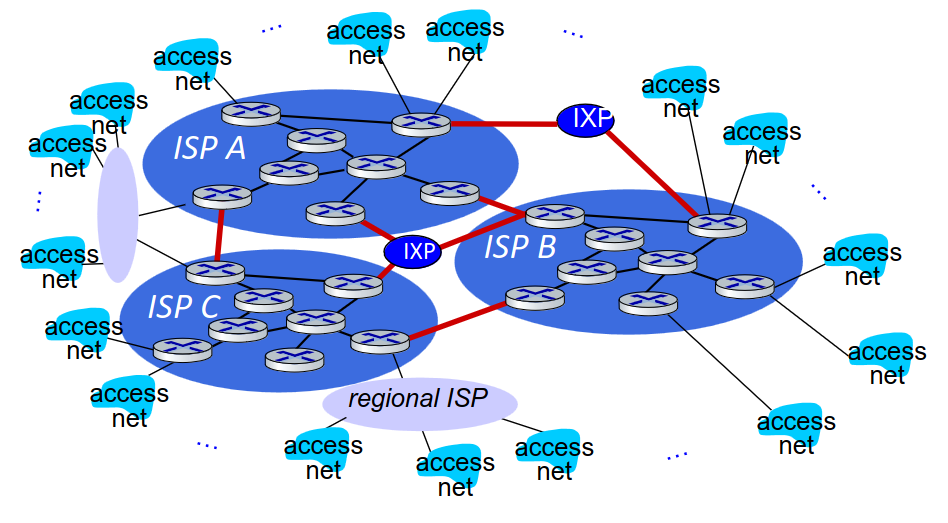
\includegraphics[scale=0.35]{Immagini/Rete-di-Reti.png}
        \caption{Struttura della rete Internet}
    \end{figure}
    
        \section{Commutazione e Ritardi}

    \begin{definition}[Commutazione]
        Modalità con cui viene determinato il percorso sorgente-destinazione e vengono dedicate ad esso le risorse della rete.
    \end{definition}

    Esistono due meccanismi:
    \begin{itemize}
        \item \textcolor{purple}{Commutazione di Circuito}
        \item \textcolor{purple}{Commutazione di Pacchetto}
    \end{itemize}

    \paragraph{Metriche}Data una comunicazione tra due host, indipendentemente dal tipo di commutazione utilizzata, è possibile utilizzare delle metriche comuni per l'analisi delle prestazioni:
    \begin{itemize}
        \item \textcolor{purple}{Bandwidth:} larghezza dell’intervallo di frequenze utilizzato dal sistema trasmissivo (si misura in Hz).
        \item \textcolor{purple}{Transmission Rate:} quantità di dati (bits) che possono essere trasmessi per unità di tempo su un certo collegamento (dipende dal bandwidth ma anche dal mezzo trasmissivo, rumore, ecc...).
        \item \textcolor{purple}{Throughput:} quantità di dati che possono essere trasmessi con successo dalla sorgente alla destinazione in un certo intervallo di tempo al netto di perdite sulla rete (duplicazioni, protocolli, ecc...).
        \newline
        In un percorso da una sorgente a una destinazione un pacchetto può passare attraverso numerosi link, perciò il throughput dell'intero percorso è dato dal percorso intermedio con throughput minore.
    \end{itemize}

    NB: Throughput $<$ Transmission Rate
        
    \subsection{Commutazione di Circuito}   
    Nella commutazione di circuito si instaura un cammino dedicato tra i due dispositivi che vogliono comunicare. Il percorso viene stabilito all’inizio della comunicazione (\textcolor{purple}{Setup}) e vengono dedicate risorse alla comunicazione (canale logico o circuito) in modo esclusivo. Le risorse allocate sono garantite per tutta la durata della comunicazione, indipendentemente dall’utilizzo effettivo.
    \paragraph*{Canale logico} Per quanto riguarda l'assegnazione di un canale di comunicazione logico esistono due principali metodi:
        \begin{itemize}
            \item \textbf{\textcolor{purple}{FDM}}: Frequency Division Multiplexing, il canale di comunicazione viene suddiviso in bande di frequenze ognuna delle quali viene assegnata in modo esclusivo ad una certa connessione.
            \item \textbf{\textcolor{purple}{TDM}}: Time Division Multiplexing, il tempo viene suddiviso in slot di tempo. Ogni comunicazione ha uno o più slot periodici assegnati nei quali può trasmettere alla velocità massima del canale.
        \end{itemize}

    \paragraph*{Vantaggi:}
    \begin{itemize}
        \item Performance garantite.
        \item Tecnologie di switching efficienti.
    \end{itemize}

    \paragraph*{Svantaggi:}
    \begin{itemize}
        \item Necessaria una fase di instaurazione della comunicazione.
        \item le risorse rimangono inattive se non utilizzate (non c’è condivisione).
    \end{itemize}


    \subsection{Commutazione di Pacchetto}
    Nella commutazione di pacchetto il flusso di dati punto-punto viene suddiviso in pacchetti. Ogni pacchetto è instradato singolarmente e indipendentemente dagli altri pacchetti della stessa comunicazione (possono seguire lo stesso percorso o percorsi diversi in base alle necessità).
    \newline
    I commutatori (es. router) devono ricevere integralmente i pacchetti prima di poterne continuare l'instradamento. Quando ci sono più pacchetti in ingresso ripetto a quanto il canale può supportare, questi vengono messi in coda in dei buffer (se il buffer è pieno i pacchetti vengono persi).
    
    \paragraph*{Vantaggi:}
    \begin{itemize}
        \item Risorse trasmissive usate solo se necessario.
        \item Fase di setup e segnalazione della connessione non richiesta.
    \end{itemize}

    \paragraph*{Svantaggi:}
    \begin{itemize}
        \item Tecnologie di inoltro poco effienti (calcolo del percorso indipendente per ogni pacchetto).
        \item Ritardi variabili nel percorso end-to-end (jitter).
        \item protocolli necessari per un trasferimento dati affidabile, controllo della congestione.
    \end{itemize}

    \subsection{Ritardi}

    \begin{definition}[Latenza] 
        Tempo richiesto affinché un messaggio arrivi a destinazione dal momento in cui il primo bit parte dalla sorgente.
    \end{definition}

    Il valore della latenza in una rete a commutazione di pacchetto è determinato da 4 tipologie di ritardo:
    \begin{itemize}
        \item \textcolor{purple}{Ritardo di eleborazione}, dovuto ai controlli di errore sui bit e dal calocolo del percorso di uscita del pacchetto.
        \item \textcolor{purple}{Ritardo di accodamento}, dovuta all'attesa dei pacchetti nel buffer la quale dipende dal tipo e dall'intensità del traffico.
        \item \textcolor{purple}{Ritardo di trasmissione:}, tempo impiegato per trasmettere un pacchetto sul canale. 
        \newline Dipende da due valori
        \begin{itemize}
            \item \textcolor{blue}{R}, rate di trasmissione sul canale (in bps).
            \item \textcolor{blue}{L}, lungezza del pacchetto (in bit).
        \end{itemize}
        Si calcola come \textcolor{blue}{L/R}.
        \item \textcolor{purple}{Ritardo di propagazione}, tempo impiegato da 1 bit per essere propagato da un nodo all’altro
        \newline Dipende anch'esso da due valori
        \begin{itemize}
            \item \textcolor{blue}{d}, lunghezza del collegamento fisico (in metri).
            \item \textcolor{blue}{s}, velocità di propagazione del mezzo.
        \end{itemize}
        Si calcola come \textcolor{blue}{d/s}.
    \end{itemize}
    
    La latenza è quindi la somma di tutti questi 4 ritardi. Nella pratica però i ritardi di elaborazione e accodamento vengono trascurati e la latenza end-to-end è data dalla somma dei ritardi di propagazione e trasmissione di tutti i collegamenti intermedi.
        \section{Modelli Stratificati}
\subsection{Perché e come stratificare}
Nei sistemi di comunicazione non si utilizza un unico protocollo infatti, stratificare il problema permette di:
\begin{itemize}
    \item scomporre il problema in sottoproblemi più semplici da trattare; il singolo strato è più semplice del sistema nel suo complesso.
    \item semplificare la progettazione, implementazione e manutenzione del software.
    \item rendere i livelli indipendenti: è possibile modificare l’implementazione di uno strato senza dover cambiare gli altri, a patto che l’interfaccia non cambi.
\end{itemize}

La separazione dei livelli non può ovviamente essere fatta in modo superficiale. Avere troppi livelli infatti rende il sistema poco scalabile, d'altro canto averne pochi rende i vari livelli complessi da realizzare. 
\newline Il processo di stratificazione avviene seguendo due principi:
\begin{itemize}
    \item \textbf{\textcolor{purple}{Separation of Concern}}: separazione degli interessi e delle responsabilità, fare ciò che compete, delegando ad altri tutto ciò che è delegabile.
    \item \textbf{\textcolor{purple}{Information Hiding}}: nascondere tutte le informazioni che non sono indispensabili per il committente per definire compiutamente l'operazione.
\end{itemize}
Per garantire questi due principi inoltre la comunicazione tra livelli adiacenti deve essere ridotta al minimo indispensabile e ogni strato deve svolgere una sola e ben definita funzione.

\subsection{Open System Interconnection}
\paragraph{Sistemi chiusi} Negli anni '60 nascono le prime reti di calcolatori come ARPANET\footnote{\url{https://it.wikipedia.org/wiki/ARPANET}}, SNA (IBM)\footnote{\url{https://it.wikipedia.org/wiki/Systems_Network_Architecture}} e DNA (Digital) che utilizzano architetture di rete a strati. Ognuna di queste reti però utilizzava protocolli proprietari incapaci di operare in ambienti condivisi perché non in grado di interpretare i segnali provenienti dall'esterno.

\paragraph{Sistemi aperti} L'obiettivo principale di questa tipologia di sistemi e quello di realizzare una rete di calcolatori in cui qualsiasi terminale comunica con un qualunque fornitore di servizi mediante una rete. \newline Per poter rendere possibile questo obiettivo è necessario stabilire delle regole comuni, degli \textcolor{purple}{standard}.

\begin{definition}
    Un protocollo è detto \textbf{\textcolor{purple}{Aperto}} se:
    \begin{itemize}
        \item i dettagli sono disponibili pubblicamente.
        \item i cambiamenti sono gestiti da un'organizzazione la cui partecipazione è aperta al pubblico.
    \end{itemize}
\end{definition}
\begin{definition}
    Un sistema che implementa protocolli aperti è un \textbf{\textcolor{purple}{Sistema Aperto}} (Open System)
\end{definition}

L’International Organization for Standards (ISO) ha specificato uno standard per l’interconnessione di sistemi aperti denominato Reference Model Open System Interconnection (\textcolor{purple}{OSI RM}).

\begin{definition}[Strato] 
    È un modulo interamente definito attraverso i servizi, protocolli e le interfacce che lo caratterizzano.
\end{definition}
\begin{definition}[Servizio]
    Servizi che uno strato fornisce ad uno strato soprastante attraverso primitive di servizio.
\end{definition}
\begin{definition}[Interfaccia]
    Insieme di regole che governano il formato e il significato delle unità di dati (es. messaggi, segmenti o pacchetti) che vengono scambiati tra due strati adiacenti della stessa entità.
\end{definition}
\begin{definition}[Protocollo]
    Insieme di regole che definiscono il formato e l’ordine dei messaggi inviati e ricevuti tra entità omologhe della rete e le azioni che vengono fatte per la trasmissione e ricezione dei messaggi; in modo:
    \begin{itemize}
        \item \textcolor{purple}{Efficace:} Un sistema che riesce a raggiungere lo scopo prefissato con la maggior frequenza possibile.
        \item \textcolor{purple}{Efficiente:} Un sistema che riesce a raggiungere lo scopo prefissato con il minor sforzo possibile.
    \end{itemize}
    
\end{definition}

\paragraph{Cosa deve fare un protocollo} In un protocollo vanno specificati:
\begin{itemize}
    \item La sintassi del messaggio: che campi contiene e in quale formato.
    \item La semantica del messaggio: come interpretare i vari campi e il messaggio stesso.
    \item Le azioni da intraprendere dopo la ricezione di un messaggio.
\end{itemize}

\newpage

\subsection{Gerarchia degli strati ISO/OSI}
\begin{figure}[h]
    \centering
    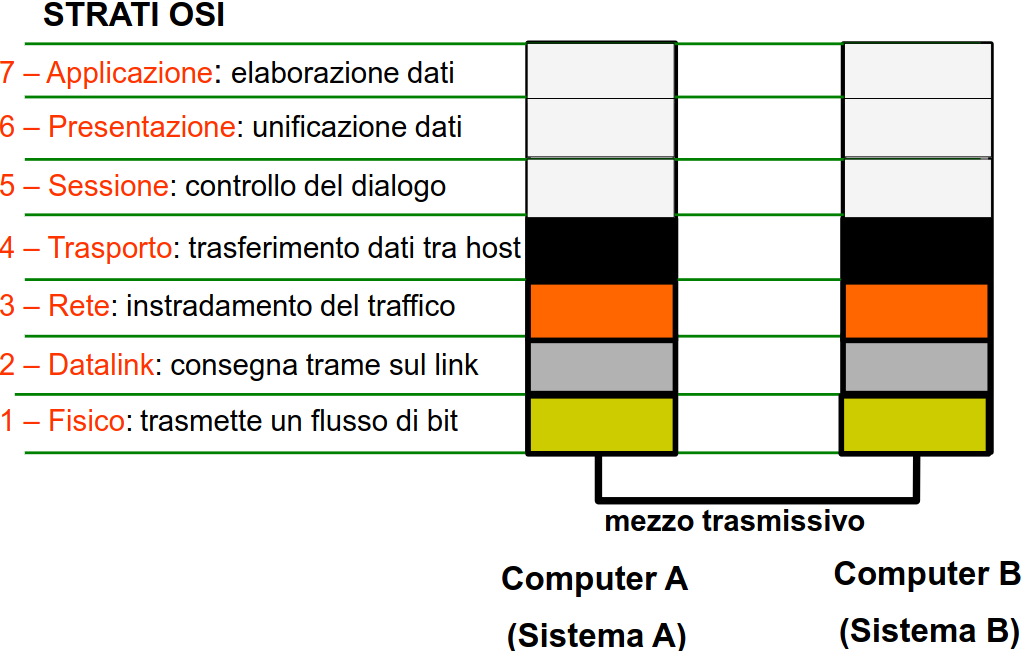
\includegraphics[scale=0.34]{Immagini/Strati_modello_ISO-OSI.png}
    \caption{Strati definiti nel modello ISO/OSI}
\end{figure}
\begin{itemize}
    \item \textbf{\textcolor{purple}{Livello Fisico:}} 
        \begin{itemize}
        \item Comprende tutte le funzioni (procedure meccaniche ed elettroniche) che permettono una connessione a livello fisico.
        \item Si occupa della trasmissione dei bit attraverso il mezzo trasmissivo e delle caratteristiche di cavi e connettori.
        \end{itemize}
    \item \textbf{\textcolor{purple}{Livello di Collegamento:}} 
        \begin{itemize}
            \item Definisce le regole per inviare e ricevere informazioni tra due sistemi in comunicazione.
            \item Si occupa di formare i dati da inviare attraverso il livello fisico, incapsulando i dati in un pacchetto provvisto di header (intestazione) e tail (coda), chiamato frame.
        \end{itemize}
    \item \textbf{\textcolor{purple}{Livello di Rete:}}
        \begin{itemize}
            \item Deve far giungere i “pacchetti” a destinazione.
            \item Si occupa dell’istradamento (“routing”) dei pacchetti, cioè di determinare la sequenza di collegamenti punto-punto necessari per trasmettere un pacchetto da un nodo generico della rete a un altro.
        \end{itemize}
    \item \textbf{\textcolor{purple}{Livello di Trasporto:}}    
        \begin{itemize}
            \item Questo strato fornisce un servizio di trasferimento dati end-to-end.
            \item Si occupa di instaurare, mantenere e terminare una connessione.
            \item Può offrire funzionalità per frammentare e riassemblare i dati, rilevare e correggere gli errori, controllare il flusso dei dati.
        \end{itemize}
    \item \textbf{\textcolor{purple}{Livello di Sessione:}} assembla il dialogo tra nodi in unità logiche.
    \item \textbf{\textcolor{purple}{Livello di Presentazione:}} adatta la sintassi dei dati di ciascuna applicazione alla sintassi richiesta dalla sessione.
    \item \textbf{\textcolor{purple}{Livello di Applicazione:}} protocolli a supporto di applicazioni distribuite.
\end{itemize}

\begin{figure}[h]
    \centering
    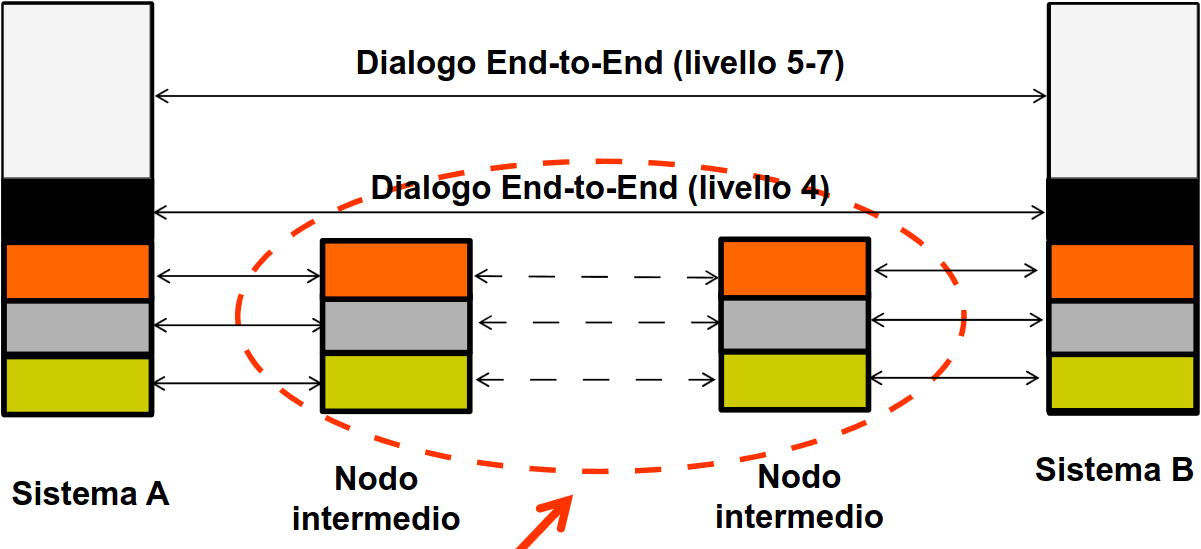
\includegraphics[scale=0.30]{Immagini/Collegamento-End-System.png}
    \caption{Collegamento tra End-System}
\end{figure}

\paragraph{Modalità di Servizio} Esistono due principali metodologie di funzionamento per la comunicazione:
\begin{itemize}
    \item \textbf{\textcolor{purple}{Connection-Oriented:}} 
        \begin{itemize}
            \item Associazione logica tra due o più sistemi al fine di trasferire dati.
            \item Gestione della connessione:
                \begin{itemize}
                    \item Instaurazione della connessione.
                    \item Trasferimento dati.
                    \item Chiusura della connessione
                \end{itemize}
        \end{itemize}
    \item \textbf{\textcolor{purple}{Connection-Less:}} I dati vengono trasferiti senza l'instaurazione di una connessione.
\end{itemize}

\paragraph{Flusso dell'informazione}
Dal punto di vista delle rete, le informazioni hanno tutte origine dal livello Applicativo. L'informazione discende i vari livelli fino alla trasmissione sul canale fisico.
Ogni livello aggiunge all’informazione del livello superiore una propria sezione informativa (o più) denominata header, che contiene informazioni riguardanti esclusivamente quel livello.
\newline Per i dati ricevuti si segue il cammino inverso.

\paragraph{Incapsulamento} Il processo di incapsulamento, ovvero quello nel quale ogni strato aggiunge dell'informazione a quella già presente, è un processo reversibile che garantisce l'estrazione durante la risalita delle informazioni dal livello di rete al livello applicativo (o fino ad un livello inferiore se ci troviamo in un nodo intermedio).
\newline In questo processo abbiamo:
\begin{itemize}
    \item \textcolor{purple}{Header:} Contente informazioni relative a quel livello.
    \item \textcolor{purple}{Payload:} Dati provenienti dal livello superiore.
    \item \textcolor{purple}{Tail:} Generalmente utilizzato per l'individuazione e la correzione degli errori.
\end{itemize}
\newpage
\begin{figure}[h]
    \centering
    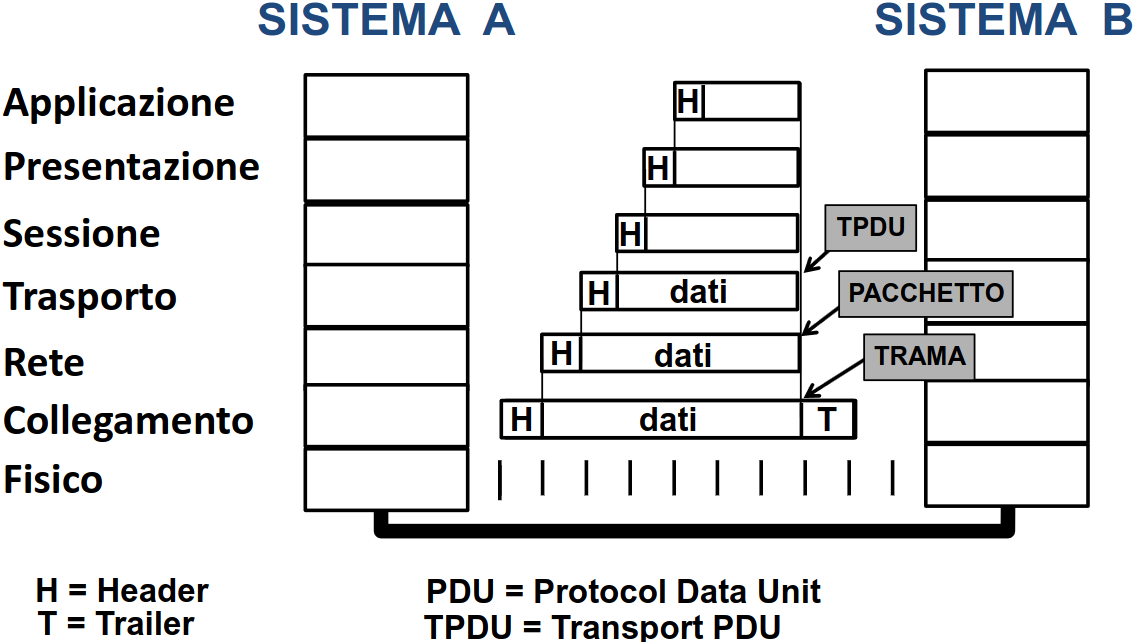
\includegraphics[scale=0.30]{Immagini/Incapsulamento-dati.png}
    \caption{Processo di incapsulamento}
\end{figure}

\subsection{Stack TCP/IP}
TCP/IP è una famiglia di protocolli attualmente utilizzata in Internet. Si tratta di una gerarchia di protocolli, ciascuno dei quali fornisce funzionalità specifiche.
\newline Definita in origine in termini di quattro livelli software soprastanti a un livello hardware, la pila TCP/IP è oggi intesa come composta di cinque livelli.
\begin{itemize}
    \item \textbf{\textcolor{purple}{Applicazione:}} supporta le applicazioni di rete, collegamento logico end-to-end; scambio di messaggi tra due processi (ftp, smtp, http).
    \item \textbf{\textcolor{purple}{Trasporto:}} trasferimento dati end-to-end da un host sorgente all’host destinatario (tcp, udp).
    \item \textbf{\textcolor{purple}{Rete:}} instradamento dei datagrammi dalla sorgente alla destinazione (Ip, ICMP).
    \item \textbf{\textcolor{purple}{Link:}} trasferimento dati in frame attraverso il collegamento tra elementi di rete vicini (p2p, ethernet, ...).
    \item \textbf{\textcolor{purple}{Fisico:}} trasferimenti dei bit di un frame sul mezzo trasmissivo.
\end{itemize}

\paragraph{Differenze tra ISO/OSI e TCP/IP} Nella pratica in Internet viene utilizzato lo stack protocollare TCP/IP. Questo accade perché ISO/OSI, a differenza di TCP/IP, fornisce una specifica generale, difficile da implementare e poco efficiente. ISO/OSI però viene utilizzato ancora come modello di riferimento.
        \section{Lo strato Applicativo}
\paragraph{Applicazioni} 
Le applicazioni di rete sono formate da processi distributi, su vari host. Ogni host può eseguire uno o più processi contemporaneamente. Questi processi comunicano tra loro mediante lo scambio di \textcolor{purple}{messaggi}.
\newline I livelli applicazione nei due lati della comunicazione agiscono come se esistesse un collegamento diretto su cui inviare questi messaggi.
\newline Il protocolli del livello applicativo definicono:
\begin{itemize}
    \item il tipo dei messaggi (es: di richiesta e di risposta).
    \item la sintassi dei vari tipi di messaggio (i campi del messaggio).
    \item la semantica dei campi (significato).
    \item le regole per determinare quando e come un processo invia messaggi o risponde ai messaggi.
\end{itemize}

\paragraph{Paradigmi del livello applicativo} Il modo in cui gli host devono comportarsi quando utilizzano una certa applicazione di rete dipende dal tipo di paradigma che questa applicazione utilizza:
\begin{itemize}
    \item \textbf{\textcolor{purple}{Client-Server:}} Un numero limitato di host, detti \textcolor{purple}{Server}, offrono servizi e sono sempre in attesa di richieste; al contrario, i restanti host, detti \textcolor{purple}{Client}, inviano richieste ai server per ricevere servizi.
    \item \textbf{\textcolor{purple}{Peer-to-Peer:}} Tutti gli host che utilizzano l'applicazione sono allo "pari" tra loro, tutti chiedono e ricevono servizi da tutti gli altri.
    \item \textbf{\textcolor{purple}{Misto}}
\end{itemize}

\begin{definition}[API]
    \textcolor{purple}{Application Programming Interface} Insieme di regole che un programmatore deve rispettare per utilizzare delle risorse.
\end{definition}

\paragraph{Interfaccia Socket} L'inteerfaccia socket (l'API di internet per eccellenza) e quell'interfaccia che si frappone tra il livello di applicazione e il livello di trasporto. Questa interfaccia è messa a disposizione dal sistema operativo che impolementa i 4 livelli inferiori dello stack protocollare TCP/IP.
La socket è una struttura dati formata da:
\begin{itemize}
    \item \textcolor{purple}{Indirizzo IP}: identificativo della macchina con cui vogliamo comunicare (32bit per indirizzi ipv4, 128bit per indirizzi ipv6);
    \item \textcolor{purple}{Porta}: numero a 16 bit che permette di identificare il processo sulla macchina con il quale si vuole comunicare.
\end{itemize} 

\subsection{Protocolli TCP e UDP}
Nel livello di trasporto della pila di protocolli TCP/IP i due protocolli principali sono:
\begin{itemize}
    \item \textbf{\textcolor{purple}{TCP:}} (Transmission Control Protocol) Protocollo connection-oriented, richiede una fase di setup tra client e server, che garantisce un trasporto affidabile dei dati. Fornisce inoltre meccaniscmi di controllo del flusso (il mittente non inonda il destinatario di dati) e della congestione (il mittente viene "rallentato" in caso di congestione della rete).
    \item \textbf{\textcolor{purple}{UDP:}} (User Datagram Protocol) Protocollo connection-less, non necessità di una fase di setup. Non garantisce trasporto affidabile e non presenta controlli di alcun tipo su flusso e congestione.
\end{itemize}
NB: entrambi \underline{non} forniscono garanzie di timing e banda minima.
\newline
\newline La scelta del protocollo da utilizzare dipende dalle esigenze dell'applicazione:
\begin{itemize}
    \item \textcolor{purple}{Throughput}: quanto è importante avere un certo livello di throughput per l'applicazione?
    \item \textcolor{purple}{Perdita dei dati}: il 100$\%$ dei dati trasferiti devono necessariamente arrivare a destinazione?
    \item \textcolor{purple}{Sensibilità ai ritardi}: l'applicazione è di tipo real-time?
\end{itemize}

\subsection{URI, URL E URN}
\paragraph{URI} Uniform Resource Identifier, è una forma generale per identificare una risorsa presente in rete:
\begin{itemize}
    \item \textcolor{purple}{Uniform}: uniformità della sintassi dell’identificatore, anche con meccanismi diversi di accesso;
    \item \textcolor{purple}{Resource}: qualsiasi cosa abbia un'identità (documento, servizio, immagine...);
    \item \textcolor{purple}{Identifier}: informazioni che permettono di distinguere un oggetto dagli altri.
\end{itemize} 
Esistono due principali tipologie di URI:
\begin{itemize}
    \item \textbf{\textcolor{purple}{URL:}} (Uniform Resource Locator) sottoinsieme di URI che identifica  le risorse attraverso il loro meccanismo di accesso.
    \item \textbf{\textcolor{purple}{URN:}} (Uniform Resource Name) sottoinsieme di URI che devono rimanere globalmente unici e persistenti anche quando la risorsa cessa di esistere e diventa non disponibile.
\end{itemize}

\paragraph{URL} Schema di una URL:
\newline $<$scheme$>$://$<$user$>$:$<$password$>$@$<$host$>$:$<$port$>$/$<$path$>$
\begin{itemize}
    \item $<$user$>$ e $<$password$>$ opzionale, in generale deprecato;
    \item $<$scheme$>$ indica il protocollo di accesso alla risorsa;
    \item $<$host$>$ nome di dominio di un host o indirizzo ip (in notazione decimale puntata);
    \item $<$port$>$ numero di porta del server;
    \item $<$path$>$ contiene dati specifici per l’host (o scheme) e identifica la risorsa nel contesto di quello schema e host.
\end{itemize}
A loro volta le URL possono essere di due tipologie differenti:
\begin{itemize}
    \item \textcolor{purple}{URL assoluta:} identifica una risorsa indipendentemente dal contesto in cui è usata;
    \item \textcolor{purple}{URL relativa:} informazioni per identificare una risorsa in relazione ad un’altra URL (è priva dello schema e della authority).
\end{itemize}
Le URL relative non vengono utilizzate in rete, ma vengono interpretate dal browser in relazione al documento di partenza.

\subsection{HTTP}
\paragraph{HyperText Transfer Protocol} Protocollo di tipo richiesta/risposta nel quale un client inizia la connessione, inviando al server una \textcolor{purple}{request}, e ricevendo da esso una \textcolor{purple}{response}. 
HTTP viene detto \textcolor{purple}{stateless} inquanto ogni coppia richiesta/risposta è indipendente da tutte le altre. 
Per funzionare utilizza il protocollo di trasporto TCP con il quale viene instaurata una connessione tra client e server.

\begin{definition}[Connessione]
    Un circuito logico, al livello di trasporto, stabilito tra due programmi applicativi per comunicare tra loro.    
\end{definition}
\begin{definition}[Connessione non persistente, da RFC 1945]
    Viene stabilita unaconnessione TCP separata per recuperare ciascuna URL.
\end{definition}
\begin{definition}[Connessione persistente, da RFC 2616]
    Se non diversamente indicato, il client può assumere che il server manterrà una connessione persistente.
    \begin{itemize}
        \item Lo standard specifica un meccanismo con cui client e server possono indicare la chiusura della connessione TCP (Connection header field);
        \item Dopo la chiusura, il client non deve più inviare richieste su quella connessione.
    \end{itemize}
\end{definition}

\newblock

\begin{figure}
    \centering
    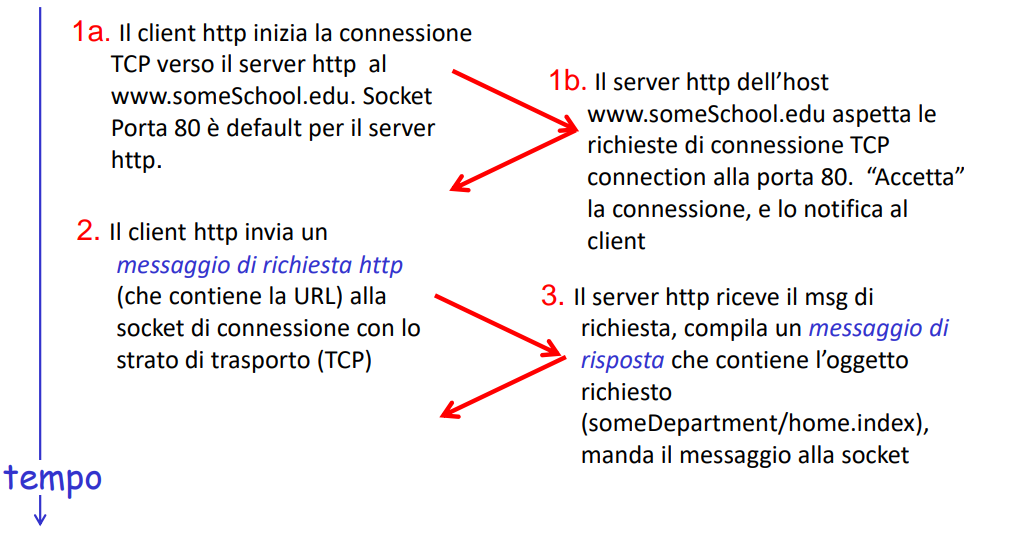
\includegraphics[scale=0.35]{Immagini/Esempio_richiesta_HTTP.png}
    \caption{Esempio di interazione con protocollo HTTP (1)}
\end{figure}

\begin{figure}[h]
    \centering
    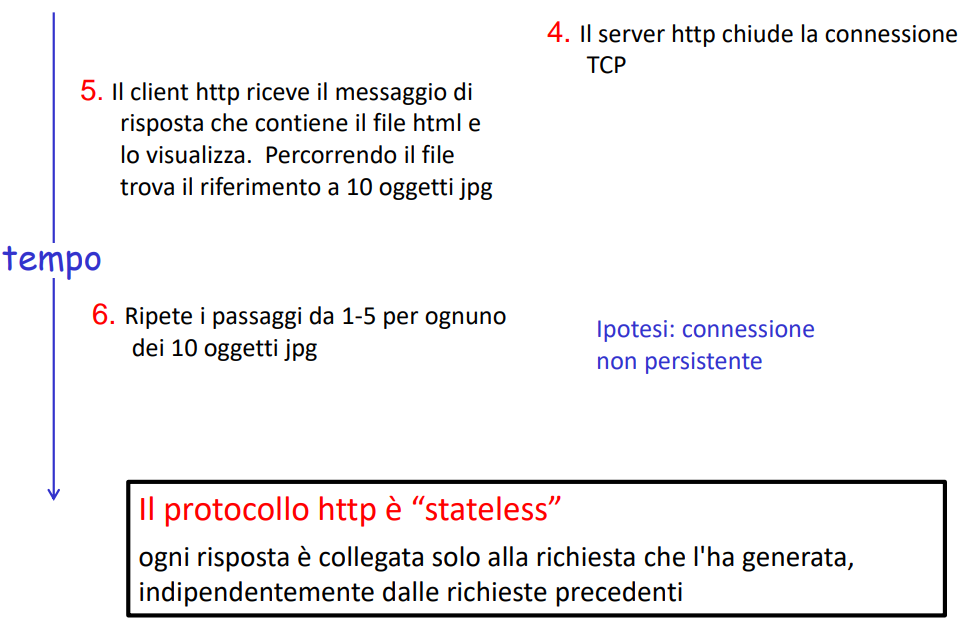
\includegraphics[scale=0.35]{Immagini/Esempio_richiesta_HTTP_2.png}
    \caption{Esempio di interazione con protocollo HTTP (2)}
\end{figure}

In caso di connessione persistente, questa non può essere utilizzata per una serie di richieste ed una corrispondente serie di risposte. Il server infatti dopo aver inviato la sua risposta rimane in attesa di altre richieste sulla connessione già aperta, fino ad una richiesta di chiusura da parte del client (che lo specifica nell'header) o in caso di attesa prolungata (time out).

    \end{sloppypar}

\end{document}  